\documentclass{tufte-handout}
\usepackage{amsmath}
\pagestyle{empty}
\usepackage[utf8]{inputenc}
\usepackage{mathpazo}
\usepackage{microtype}

\usepackage{tikz}
\usetikzlibrary{matrix}
\usetikzlibrary{chains}
\usetikzlibrary{decorations}

\title{Gorilla or Sea Cucumber?}
\author{Thore Husfeldt}

\begin{document}

\maketitle

\subsection{Description}
Implement the dynamic programming sequence alignment algorithm and run it on some realistic protein sequences.

\begin{marginfigure}
  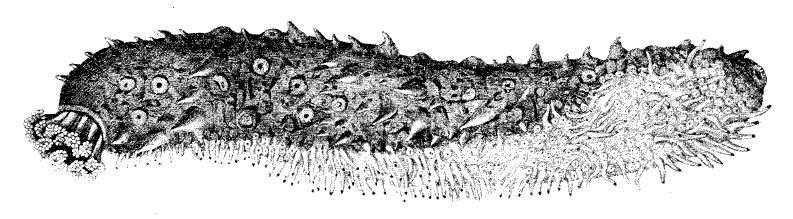
\includegraphics[width=2in]{sea_cucumber.png}
  \caption{A sea cucumber. Ugly bastard.
  Image from \emph{Nordisk familjebok}, 1876.}
\end{marginfigure}

\subsection{Requirements}

Your algorithm computes both the score and the proper alignment of a number of species given in the file \verb!HbB_FASTAs-in.txt!,
using the dynamic programming idea for sequence alignment\sidenote{\S 6.6 of Kleinberg and Tardos, \emph{Algorithms Design}, Addison--Wesley (2006).}
The mismatch costs $\alpha_{pq}$ and gap penalty $\delta$ are given in the file \verb!BLOSUM62.txt!.

Quadratic space is fine.

Your code must read the input ``FASTA'' data from a file or standard input and must write to standard output.
The costs (in the ``BLOSUM'' file) you can open as a file, or even hard-code it into your program if you find that easier.


\subsection{Tips}

The BLOSUM matrix is taken from a computational biology source.
You need to stare a bit at the BLOSUM matrix in order to make sense of it.
Note that the scores in the BLOSUM matrix are large for good alignments, and small for bad ones.
That is the opposite convention from what is assumed in the book, so you either need to change signs in the matrix, or use ``max'' instead of ``min''.\sidenote{I chose the latter.}
You can decide yourself if you want to use a recursive or bottom-up solution.\sidenote{I did the latter, and came to become pretty annoyed with it.}
Reporting just the score is easy enough in the bottom-up solution.
But I think the recursive approach is easier if you actually need to report an optimal alignment.
See for yourself.


\subsection{Deliverables}

\begin{enumerate}
  \item The source code for your implementation
  \item A report in PDF.
  Use the report skeleton in the {\tt doc} directory.
  \end{enumerate}

\end{document}
